\section{Products}

Die Produktseite erlaubt es, Produkte im Sokka-System hinzuzufügen, zu bearbeiten und zu löschen.

\begin{figure}[ht]
    \centering
    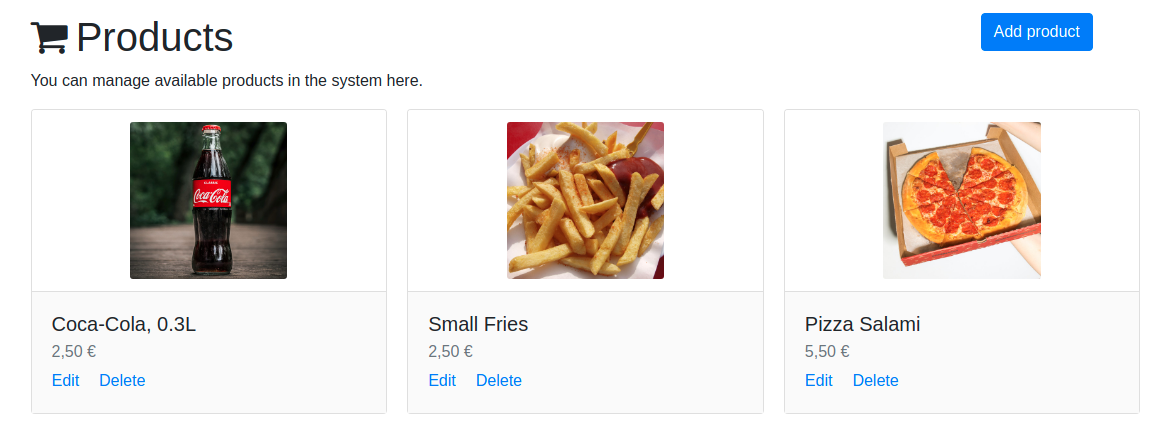
\includegraphics[width=0.8\textwidth]{images/ACP/products.png}
    \caption{Die Produkteseite des Sokka-ACPs}
\end{figure}

Die Seite zum Hinzufügen von Produkten (erreichbar über den \glqq Add product\grqq -Button) und dem Bearbeiten von Produkten (erreichbar über den \glqq Edit\grqq -Button in den einzelnen Produktkarten) baut auf derselben React-Component auf, weshalb das Aussehen der beiden Seiten nahezu identisch ist.

Die verfügbaren und einstellbaren Eigenschaften für Produkte sind:

\begin{itemize}
    \item \textbf{Name}: Der Name des Produkts
    \item \textbf{Price}: Der Preis des Produkts in Euro
    \item \textbf{Category}: Die Kategorie des Produkts
    \item \textbf{Hidden}: Ob das Produkt dem Nutzer angezeigt werden soll
    \item \textbf{Image}: Das Vorschaubild des Produkts
\end{itemize}

\begin{figure}[ht]
    \centering
    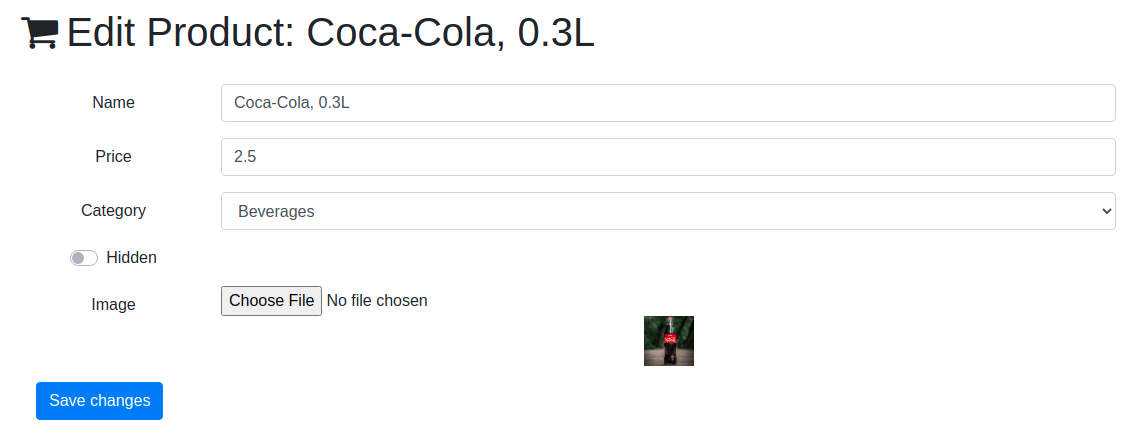
\includegraphics[width=0.8\textwidth]{images/ACP/products_edit.png}
    \caption{Die Bearbeitungsseite von Produkten im Sokka-ACP}
\end{figure}